% So I have up to 11 texts I need to show here
% lut64
% pext64
% shuffle64
% shuffle128
% shuffle256
% shuffle512
% pc
% pc-ss
% ps
% kaneta-pext
% kaneta-pshufb

\documentclass[a4]{article}

\usepackage[utf8]{inputenc}
\usepackage[english]{babel}

\usepackage{amsmath,amsfonts,amssymb}
\usepackage{fullpage}
\usepackage{verbatim}

\usepackage{tikz,pgfplots}
\usetikzlibrary{patterns, patterns.meta}
\usepgfplotslibrary{groupplots}



\pgfplotsset{
    major grid style = { thin, dotted, color = black!50 },
    minor grid style = { thin, dotted, color = black!50 },
    grid,
    xtick distance = 1,
    ymin = 0,
    legend cell align = left,
    legend pos = north west,
	  /pgfplots/ybar legend/.style = {
		  /pgfplots/legend image code/.code={%
			  \draw[##1,/tikz/.cd,yshift=-0.35em]
      (0cm,0cm) rectangle (0.7em,0.8em);},
	  },  
}


\begin{document}

\title{WT Benchmark}
\author{Jan-Philipp Tarnowski}
\maketitle

\clearpage

% Okay, this will be fun

% IMPORT-DATA stats ../results-pcc-huff-sans-sources-pitches.out
% IMPORT-DATA stats_b ../results-pcc-huff-sources.out
% IMPORT-DATA stats_c ../results-pcc-huff-pitches-no-wm-pc.out
% IMPORT-DATA stats_d ../results-lightweight-huff-chr22-gcc-30-jdk13c-rfc-w3c-rctail96.out
% IMPORT-DATA stats_e ../results-lightweight-huff-etexthowto-linux-sans-wx-pc.out
% IMPORT-DATA stats_f ../results-lightweight-huff-sprot.out


% SQL INSERT INTO stats SELECT * FROM stats_b
% SQL INSERT INTO stats SELECT * FROM stats_c
% SQL INSERT INTO stats SELECT * FROM stats_d
% SQL INSERT INTO stats SELECT * FROM stats_e
% SQL INSERT INTO stats SELECT * FROM stats_f

% Post large texts 

% IMPORT-DATA stats_x_a ../results-huff-pcc-2.out
% IMPORT-DATA stats_x_b ../results-huff-lightweight-2.out
% IMPORT-DATA stats_x_c ../results-huff-large-mawt.out
% IMPORT-DATA stats_x_d ../results-huff-wc-large-sans-pc-matrix.out
% IMPORT-DATA stats_x_e ../results-huff-pc-wm-large.out
% ~IMPORT-DATA stats_x_f ../results-ru.out % TODO: These results are junk.

% SQL DELETE FROM stats WHERE type LIKE 'lwt%'
% SQL DELETE FROM stats WHERE type LIKE 'wm%'

% SQL INSERT INTO stats SELECT * FROM stats_x_a
% SQL INSERT INTO stats SELECT * FROM stats_x_b
% SQL INSERT INTO stats SELECT * FROM stats_x_c
% SQL INSERT INTO stats SELECT * FROM stats_x_d
% SQL INSERT INTO stats SELECT * FROM stats_x_e
% ~SQL INSERT INTO stats SELECT * FROM stats_x_f


% SQL UPDATE stats SET type = 'lwt-huff-pext-16-4', ds_order = 0 WHERE type LIKE 'lwt_huffman_pext_16_4'
% SQL UPDATE stats SET type = 'lwt-huff-shuffle-8-8', ds_order = 1 WHERE type LIKE 'lwt_huffman_shuffle_8_8'
% SQL UPDATE stats SET type = 'lwt-huff-shuffle-16-8', ds_order = 2 WHERE type LIKE 'lwt_huffman_shuffle_16_8'
% SQL UPDATE stats SET type = 'lwt-huff-shuffle-32-8', ds_order = 3 WHERE type LIKE 'lwt_huffman_shuffle_32_8'
% SQL UPDATE stats SET type = 'lwt-huff-shuffle-64-8', ds_order = 4 WHERE type LIKE 'lwt_huffman_shuffle_64_8'
% SQL UPDATE stats SET type = 'lwt-pwm-huff-pc', ds_order = 5 WHERE type LIKE 'pwm_%wx_huff_pc________tree_huffman'
% SQL UPDATE stats SET type = 'lwt-pwm-huff-pc-ss', ds_order = 6 WHERE type LIKE 'pwm_%wx_huff_pc_ss________tree_huffman'
% SQL UPDATE stats SET type = 'lwt-pwm-huff-ps', ds_order = 7 WHERE type LIKE 'pwm_%wx_huff_ps________tree_huffman'

% SQL UPDATE stats SET type = 'wm-huff-pext-16-4', ds_order = 8 WHERE type LIKE 'wm_huffman_pext_16_4'
% SQL UPDATE stats SET type = 'wm-huff-shuffle-8-8', ds_order = 9 WHERE type LIKE 'wm_huffman_shuffle_8_8'
% SQL UPDATE stats SET type = 'wm-huff-shuffle-16-8', ds_order = 10 WHERE type LIKE 'wm_huffman_shuffle_16_8'
% SQL UPDATE stats SET type = 'wm-huff-shuffle-32-8', ds_order = 11 WHERE type LIKE 'wm_huffman_shuffle_32_8'
% SQL UPDATE stats SET type = 'wm-huff-shuffle-64-8', ds_order = 12 WHERE type LIKE 'wm_huffman_shuffle_64_8'
% SQL UPDATE stats SET type = 'wm-pwm-huff-pc', ds_order = 13 WHERE type LIKE 'pwm_%wx_huff_pc________matrix_huffman'
% SQL UPDATE stats SET type = 'wm-pwm-huff-pc-ss', ds_order = 14 WHERE type LIKE 'pwm_%wx_huff_pc_ss________matrix_huffman'
% SQL UPDATE stats SET type = 'wm-pwm-huff-ps', ds_order = 15 WHERE type LIKE 'pwm_%wx_huff_ps________matrix_huffman'

% SQL DELETE FROM stats WHERE type LIKE '%\_%' ESCAPE '\'


% IMPORT-DATA text_info ../results-stats.log

% SQL CREATE TABLE stats_joined AS SELECT * FROM stats JOIN text_info ON stats.file = text_info.file
% SQL DROP TABLE stats
% SQL ALTER TABLE stats_joined RENAME TO stats

% SQL UPDATE stats SET file = 'dblp.xml' WHERE file LIKE '%/dblp.xml'
% SQL UPDATE stats SET file = 'dna' WHERE file LIKE '%/dna'
% SQL UPDATE stats SET file = 'english' WHERE file LIKE '%/english'
% SQL UPDATE stats SET file = 'pitches' WHERE file LIKE '%/pitches'
% SQL UPDATE stats SET file = 'proteins' WHERE file LIKE '%/proteins'
% SQL UPDATE stats SET file = 'sources' WHERE file LIKE '%/sources'

% SQL UPDATE stats SET file = 'chr22.dna' WHERE file LIKE '%/chr22.dna'
% SQL UPDATE stats SET file = 'etext99' WHERE file LIKE '%/etext99'
% SQL UPDATE stats SET file = 'gcc-3.0.tar' WHERE file LIKE '%/gcc-3.0.tar'
% SQL UPDATE stats SET file = 'howto' WHERE file LIKE '%/howto'
% SQL UPDATE stats SET file = 'jdk13c' WHERE file LIKE '%/jdk13c'
% SQL UPDATE stats SET file = 'linux-2.4.5.tar' WHERE file LIKE '%/linux-2.4.5.tar'
% SQL UPDATE stats SET file = 'rctail96' WHERE file LIKE '%/rctail96'
% SQL UPDATE stats SET file = 'rfc' WHERE file LIKE '%/rfc'
% SQL UPDATE stats SET file = 'sprot34.dat' WHERE file LIKE '%/sprot34.dat'
% SQL UPDATE stats SET file = 'w3c2' WHERE file LIKE '%/w3c2'

% SQL UPDATE stats SET file = 'cc.16gib' WHERE file LIKE '%/cc.txt'
% SQL UPDATE stats SET file = 'dna.16gib' WHERE file LIKE '%/dna.txt'
% SQL UPDATE stats SET file = 'wiki.16gib' WHERE file LIKE '%/wiki.txt'
% SQL UPDATE stats SET file = 'ru.8gib' WHERE file LIKE '%/ru.wo_punct.wb'

\pgfplotsset{
  /pgfplots/bar cycle list/.style = {
    /pgfplots/cycle list = {
      { fill = green!65, mark = none },        % PEXT
      { fill = blue!55, mark = none },         % PSHUFB 8-8
      { fill = orange!65, mark = none },       % PSHUFB 16-8
      { fill = violet!60, mark = none },       % PSHUFB 32-8
      { fill = yellow!80, mark = none },       % PSHUFB 64-8
      { fill = blue!50!green!75, mark = none },% PWM PC
      { fill = red!75!blue!50, mark = none },  % PWM PC SS
      { fill = brown!50, mark = none }         % PWM PS
    }
  }
}

\begin{figure}[t]
\begin{center}
    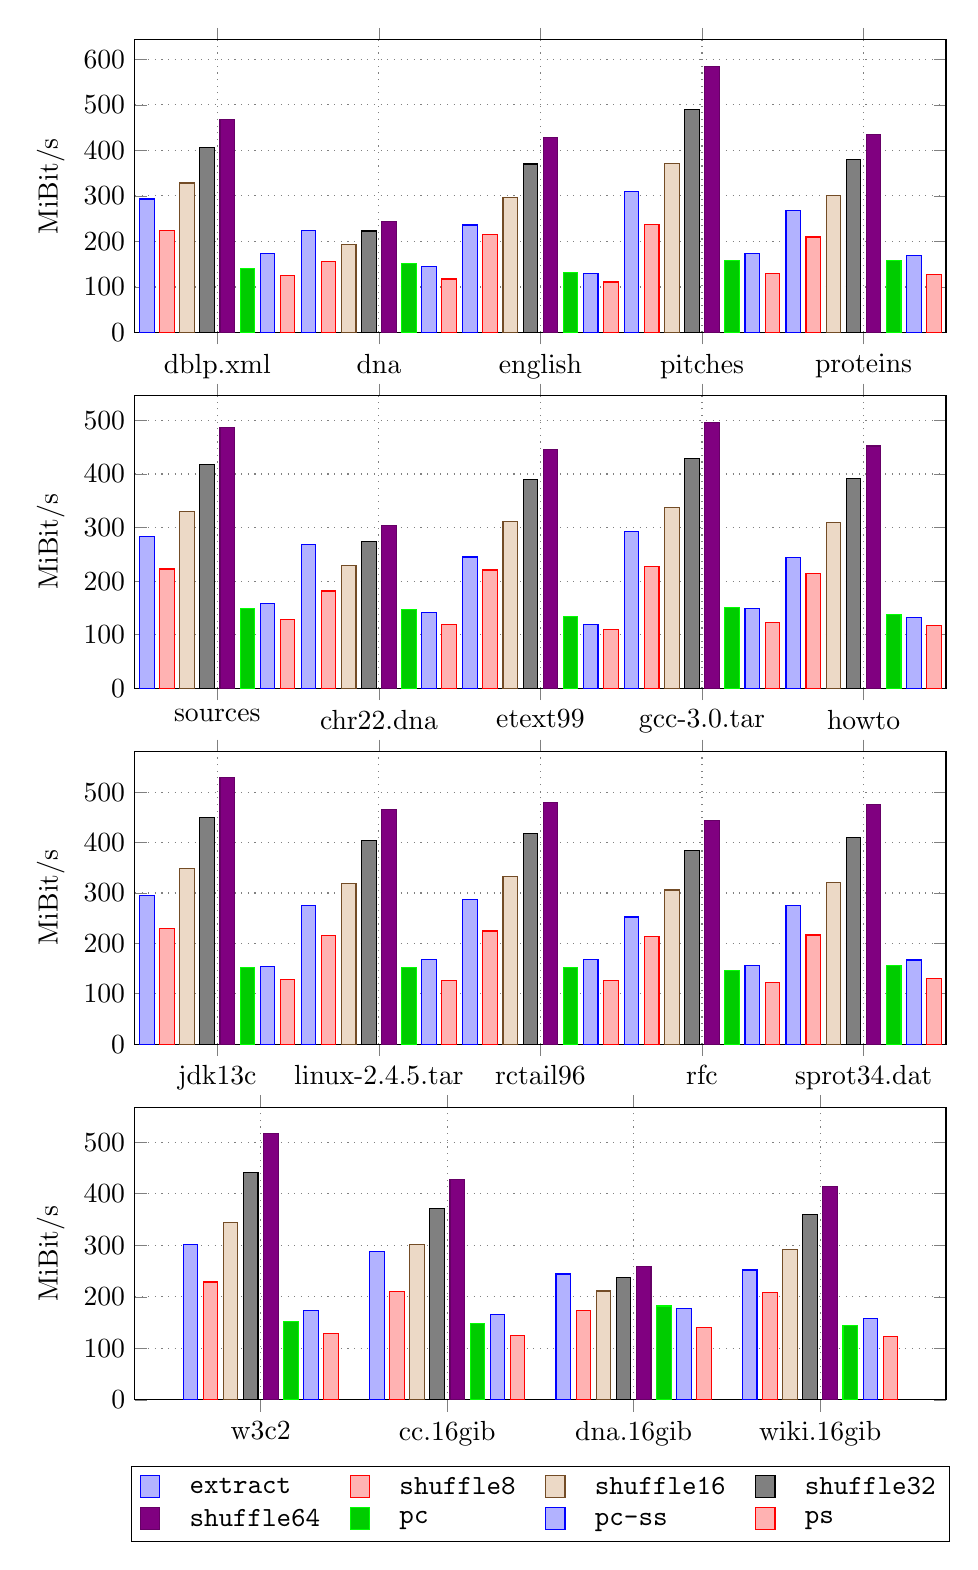
\begin{tikzpicture}
        \begin{groupplot} [
            width = 0.98\textwidth,
            height = 5.3cm,
            ybar,
            enlarge x limits = 0.1275,
            group style = { 
                vertical sep = 0.8cm,
                group size = { 
                    1 by 4
                } 
            },
            ylabel = MiBit/s,
            legend style = { 
                at = {(0.5, -0.225)},
                anchor = north,
                legend columns = 4,
                column sep = 2ex
            },
            ytick distance = 100,
            symbolic x coords = {
                dblp.xml,
                dna,
                english,
                pitches,
                proteins,
                sources,
                chr22.dna,
                etext99,
                gcc-3.0.tar,
                howto,
                jdk13c,
                linux-2.4.5.tar,
                rctail96,
                rfc,
                sprot34.dat,
                w3c2,
                cc.16gib,
                dna.16gib,
                wiki.16gib,
                ru.8gib
            }
        ]
        
        
        \nextgroupplot [
            bar width = 0.185cm
        ]


			%% MULTIPLOT(type) SELECT file AS x, MEDIAN((huff_bit_size / CAST(time_in_s AS FLOAT)) / (1024 * 1024)) AS y,MULTIPLOT
			%% FROM stats WHERE (type LIKE 'lwt%' OR type LIKE '%tree') AND (file LIKE 'dblp.xml' OR file LIKE 'dna' OR file LIKE 'english' OR file LIKE 'pitches' OR file LIKE 'proteins') GROUP BY MULTIPLOT,x ORDER BY ds_order,MULTIPLOT,x
   \addplot coordinates { (dblp.xml,293.115) (dna,223.306) (english,236.198) (pitches,308.944) (proteins,267.44) };
   \addlegendentry{type=lwt-huff-pext-16-4};
   \addplot coordinates { (dblp.xml,224.922) (dna,156.6) (english,214.509) (pitches,237.258) (proteins,209.677) };
   \addlegendentry{type=lwt-huff-shuffle-8-8};
   \addplot coordinates { (dblp.xml,328.223) (dna,192.673) (english,295.569) (pitches,372.004) (proteins,300.201) };
   \addlegendentry{type=lwt-huff-shuffle-16-8};
   \addplot coordinates { (dblp.xml,405.361) (dna,222.965) (english,370.08) (pitches,488.962) (proteins,379.163) };
   \addlegendentry{type=lwt-huff-shuffle-32-8};
   \addplot coordinates { (dblp.xml,467.217) (dna,243.467) (english,428.038) (pitches,584.301) (proteins,435.128) };
   \addlegendentry{type=lwt-huff-shuffle-64-8};
   \addplot coordinates { (dblp.xml,140.491) (dna,152.187) (english,132.161) (pitches,157.421) (proteins,158.951) };
   \addlegendentry{type=lwt-pwm-huff-pc};
   \addplot coordinates { (dblp.xml,174.341) (dna,145.947) (english,129.478) (pitches,173.363) (proteins,169.758) };
   \addlegendentry{type=lwt-pwm-huff-pc-ss};
   \addplot coordinates { (dblp.xml,125.918) (dna,117.576) (english,110.99) (pitches,129.579) (proteins,127.858) };
   \addlegendentry{type=lwt-pwm-huff-ps};

    \legend{};

   \nextgroupplot [
    bar width = 0.185cm
]


    %% MULTIPLOT(type) SELECT file AS x, MEDIAN((huff_bit_size / CAST(time_in_s AS FLOAT)) / (1024 * 1024)) AS y,MULTIPLOT
    %% FROM stats WHERE (type LIKE 'lwt%' OR type LIKE '%tree') AND (file LIKE 'sources' OR file LIKE 'chr22.dna' OR file LIKE 'etext99' OR file LIKE 'gcc-3.0.tar' OR file LIKE 'howto') GROUP BY MULTIPLOT,x ORDER BY ds_order,MULTIPLOT,x
    \addplot coordinates { (chr22.dna,269.132) (etext99,245.082) (gcc-3.0.tar,292.111) (howto,244.975) (sources,283.535) };
    \addlegendentry{type=lwt-huff-pext-16-4};
    \addplot coordinates { (chr22.dna,181.706) (etext99,220.796) (gcc-3.0.tar,227.359) (howto,214.863) (sources,222.683) };
    \addlegendentry{type=lwt-huff-shuffle-8-8};
    \addplot coordinates { (chr22.dna,229.991) (etext99,310.962) (gcc-3.0.tar,338.139) (howto,309.459) (sources,330.001) };
    \addlegendentry{type=lwt-huff-shuffle-16-8};
    \addplot coordinates { (chr22.dna,274.279) (etext99,389.996) (gcc-3.0.tar,429.167) (howto,391.523) (sources,418.477) };
    \addlegendentry{type=lwt-huff-shuffle-32-8};
    \addplot coordinates { (chr22.dna,304.497) (etext99,445.999) (gcc-3.0.tar,496.742) (howto,452.262) (sources,486.503) };
    \addlegendentry{type=lwt-huff-shuffle-64-8};
    \addplot coordinates { (chr22.dna,147.697) (etext99,133.453) (gcc-3.0.tar,151.597) (howto,138.41) (sources,149.736) };
    \addlegendentry{type=lwt-pwm-huff-pc};
    \addplot coordinates { (chr22.dna,140.865) (etext99,119.462) (gcc-3.0.tar,148.651) (howto,131.617) (sources,158.276) };
    \addlegendentry{type=lwt-pwm-huff-pc-ss};
    \addplot coordinates { (chr22.dna,119.48) (etext99,110.332) (gcc-3.0.tar,123.105) (howto,116.58) (sources,127.9) };
    \addlegendentry{type=lwt-pwm-huff-ps};

    \legend{};

    \nextgroupplot [
        bar width = 0.185cm
    ]

    
    
        %% MULTIPLOT(type) SELECT file AS x, MEDIAN((huff_bit_size / CAST(time_in_s AS FLOAT)) / (1024 * 1024)) AS y,MULTIPLOT
        %% FROM stats WHERE (type LIKE 'lwt%' OR type LIKE '%tree') AND (file LIKE 'jdk13c' OR file LIKE 'sprot34.dat' OR file LIKE 'linux-2.4.5.tar' OR file LIKE 'rctail96' OR file LIKE 'rfc') GROUP BY MULTIPLOT,x ORDER BY ds_order,MULTIPLOT,x
        \addplot coordinates { (jdk13c,294.338) (linux-2.4.5.tar,275.048) (rctail96,287.319) (rfc,252.365) (sprot34.dat,274.831) };
        \addlegendentry{type=lwt-huff-pext-16-4};
        \addplot coordinates { (jdk13c,229.075) (linux-2.4.5.tar,215.604) (rctail96,224.623) (rfc,212.992) (sprot34.dat,216.732) };
        \addlegendentry{type=lwt-huff-shuffle-8-8};
        \addplot coordinates { (jdk13c,348.682) (linux-2.4.5.tar,318.626) (rctail96,332.847) (rfc,305.978) (sprot34.dat,320.458) };
        \addlegendentry{type=lwt-huff-shuffle-16-8};
        \addplot coordinates { (jdk13c,449.869) (linux-2.4.5.tar,403.663) (rctail96,418.597) (rfc,385.286) (sprot34.dat,410.213) };
        \addlegendentry{type=lwt-huff-shuffle-32-8};
        \addplot coordinates { (jdk13c,528.494) (linux-2.4.5.tar,465.778) (rctail96,480.291) (rfc,443.152) (sprot34.dat,476.584) };
        \addlegendentry{type=lwt-huff-shuffle-64-8};
        \addplot coordinates { (jdk13c,152.621) (linux-2.4.5.tar,152.365) (rctail96,151.451) (rfc,145.778) (sprot34.dat,155.63) };
        \addlegendentry{type=lwt-pwm-huff-pc};
        \addplot coordinates { (jdk13c,154.242) (linux-2.4.5.tar,167.364) (rctail96,168.195) (rfc,155.447) (sprot34.dat,167.085) };
        \addlegendentry{type=lwt-pwm-huff-pc-ss};
        \addplot coordinates { (jdk13c,128.705) (linux-2.4.5.tar,126.757) (rctail96,126.29) (rfc,122.439) (sprot34.dat,130.747) };
        \addlegendentry{type=lwt-pwm-huff-ps};

        \legend{};


        \nextgroupplot [
            bar width = 0.185cm,
            enlarge x limits = 0.225
        ]
    
        
        
            %% MULTIPLOT(type) SELECT file AS x, MEDIAN((huff_bit_size / CAST(time_in_s AS FLOAT)) / (1024 * 1024)) AS y,MULTIPLOT
            %% FROM stats WHERE (type LIKE 'lwt%' OR type LIKE '%tree') AND (file LIKE 'w3c2' OR file LIKE 'cc.16gib' OR file LIKE 'dna.16gib' OR file LIKE 'wiki.16gib') GROUP BY MULTIPLOT,x ORDER BY ds_order,MULTIPLOT,x
            \addplot coordinates { (cc.16gib,287.724) (dna.16gib,244.315) (w3c2,302.327) (wiki.16gib,251.961) };
            \addlegendentry{type=lwt-huff-pext-16-4};
            \addplot coordinates { (cc.16gib,210.775) (dna.16gib,172.695) (w3c2,228.779) (wiki.16gib,207.71) };
            \addlegendentry{type=lwt-huff-shuffle-8-8};
            \addplot coordinates { (cc.16gib,301.709) (dna.16gib,211.345) (w3c2,344.236) (wiki.16gib,291.727) };
            \addlegendentry{type=lwt-huff-shuffle-16-8};
            \addplot coordinates { (cc.16gib,370.684) (dna.16gib,236.715) (w3c2,441.428) (wiki.16gib,359.702) };
            \addlegendentry{type=lwt-huff-shuffle-32-8};
            \addplot coordinates { (cc.16gib,427.436) (dna.16gib,258.727) (w3c2,516.473) (wiki.16gib,414.723) };
            \addlegendentry{type=lwt-huff-shuffle-64-8};
            \addplot coordinates { (cc.16gib,148.24) (dna.16gib,182.211) (w3c2,152.226) (wiki.16gib,144.614) };
            \addlegendentry{type=lwt-pwm-huff-pc};
            \addplot coordinates { (cc.16gib,166.164) (dna.16gib,177.096) (w3c2,172.773) (wiki.16gib,158.651) };
            \addlegendentry{type=lwt-pwm-huff-pc-ss};
            \addplot coordinates { (cc.16gib,124.803) (dna.16gib,139.916) (w3c2,128.308) (wiki.16gib,122.848) };
            \addlegendentry{type=lwt-pwm-huff-ps};


            \legend {
                \texttt{extract},
                \texttt{shuffle8},
                \texttt{shuffle16},
                \texttt{shuffle32},
                \texttt{shuffle64},
                \texttt{pc},
                \texttt{pc-ss},
                \texttt{ps}
            }
            


        \end{groupplot}
    \end{tikzpicture}
\end{center}
\caption{Construction time results for uncompressed trees. With the exception of cc.16gib, 512 bit construction always wins out.}
\end{figure}


\begin{figure}[t]
    \begin{center}
        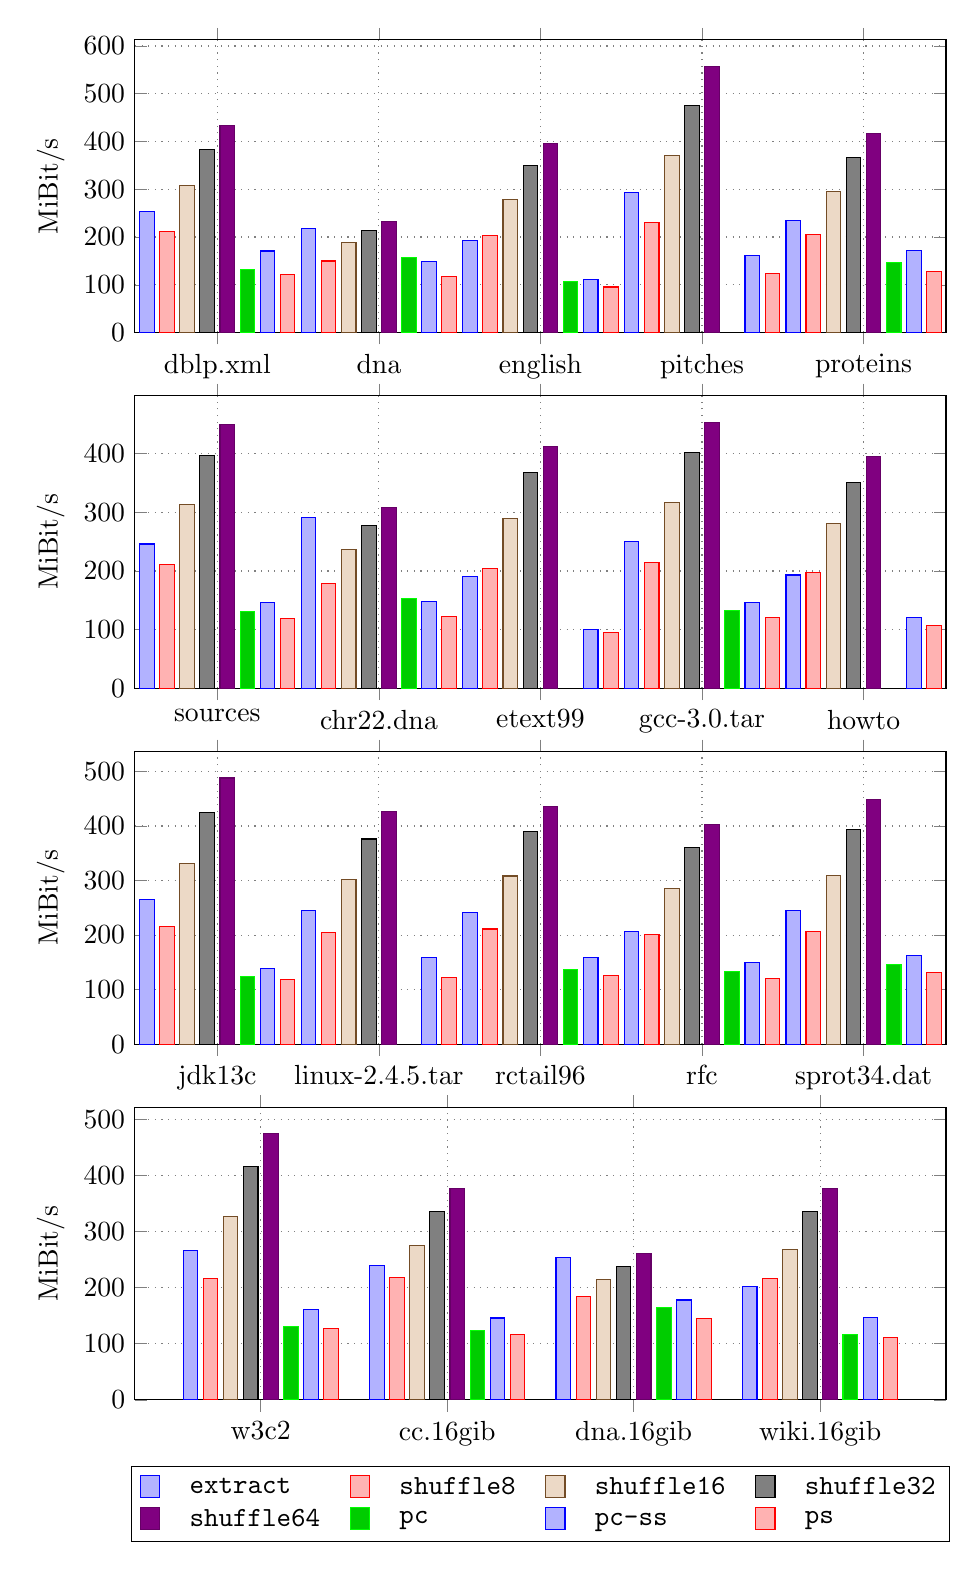
\begin{tikzpicture}
            \begin{groupplot} [
                width = 0.98\textwidth,
                height = 5.3cm,
                ybar,
                enlarge x limits = 0.1275,
                group style = { 
                    vertical sep = 0.8cm,
                    group size = { 
                        1 by 4
                    } 
                },
                ylabel = MiBit/s,
                legend style = { 
                    at = {(0.5, -0.225)},
                    anchor = north,
                    legend columns = 4,
                    column sep = 2ex
                },
                ytick distance = 100,
                symbolic x coords = {
                    dblp.xml,
                    dna,
                    english,
                    pitches,
                    proteins,
                    sources,
                    chr22.dna,
                    etext99,
                    gcc-3.0.tar,
                    howto,
                    jdk13c,
                    linux-2.4.5.tar,
                    rctail96,
                    rfc,
                    sprot34.dat,
                    w3c2,
                    cc.16gib,
                    dna.16gib,
                    wiki.16gib,
                    ru.8gib
                }
            ]
            
            
            \nextgroupplot [
                bar width = 0.185cm
            ]
    
    
                %% MULTIPLOT(type) SELECT file AS x, MEDIAN((huff_bit_size / CAST(time_in_s AS FLOAT)) / (1024 * 1024)) AS y,MULTIPLOT
                %% FROM stats WHERE (type LIKE 'wm%' OR type LIKE '%matrix') AND (file LIKE 'dblp.xml' OR file LIKE 'dna' OR file LIKE 'english' OR file LIKE 'pitches' OR file LIKE 'proteins') GROUP BY MULTIPLOT,x ORDER BY ds_order,MULTIPLOT,x
                \addplot coordinates { (dblp.xml,253.836) (dna,218.42) (english,192.703) (pitches,293.692) (proteins,233.918) };
                \addlegendentry{type=wm-huff-pext-16-4};
                \addplot coordinates { (dblp.xml,211.715) (dna,149.79) (english,202.579) (pitches,231.092) (proteins,205.349) };
                \addlegendentry{type=wm-huff-shuffle-8-8};
                \addplot coordinates { (dblp.xml,308.193) (dna,187.931) (english,278.59) (pitches,370.287) (proteins,296.245) };
                \addlegendentry{type=wm-huff-shuffle-16-8};
                \addplot coordinates { (dblp.xml,383.442) (dna,213.925) (english,350.142) (pitches,475.1) (proteins,366.709) };
                \addlegendentry{type=wm-huff-shuffle-32-8};
                \addplot coordinates { (dblp.xml,432.834) (dna,233.363) (english,396.224) (pitches,557.289) (proteins,417.439) };
                \addlegendentry{type=wm-huff-shuffle-64-8};
                \addplot coordinates { (dblp.xml,132.912) (dna,157.102) (english,106.904) (proteins,147.442) };
                \addlegendentry{type=wm-pwm-huff-pc};
                \addplot coordinates { (dblp.xml,170.812) (dna,147.899) (english,110.755) (pitches,161.067) (proteins,171.342) };
                \addlegendentry{type=wm-pwm-huff-pc-ss};
                \addplot coordinates { (dblp.xml,121.826) (dna,117.548) (english,95.3876) (pitches,123.948) (proteins,128.04) };
                \addlegendentry{type=wm-pwm-huff-ps};
    
        \legend{};
    
       \nextgroupplot [
        bar width = 0.185cm
    ]
    
    
        %% MULTIPLOT(type) SELECT file AS x, MEDIAN((huff_bit_size / CAST(time_in_s AS FLOAT)) / (1024 * 1024)) AS y,MULTIPLOT
        %% FROM stats WHERE (type LIKE 'wm%' OR type LIKE '%matrix') AND (file LIKE 'sources' OR file LIKE 'chr22.dna' OR file LIKE 'etext99' OR file LIKE 'gcc-3.0.tar' OR file LIKE 'howto') GROUP BY MULTIPLOT,x ORDER BY ds_order,MULTIPLOT,x
        \addplot coordinates { (chr22.dna,290.684) (etext99,190.628) (gcc-3.0.tar,250.542) (howto,193.264) (sources,246.025) };
        \addlegendentry{type=wm-huff-pext-16-4};
        \addplot coordinates { (chr22.dna,179.097) (etext99,204.71) (gcc-3.0.tar,215.271) (howto,197.022) (sources,211.239) };
        \addlegendentry{type=wm-huff-shuffle-8-8};
        \addplot coordinates { (chr22.dna,236.764) (etext99,289.381) (gcc-3.0.tar,317.078) (howto,281.024) (sources,313.175) };
        \addlegendentry{type=wm-huff-shuffle-16-8};
        \addplot coordinates { (chr22.dna,278.319) (etext99,367.3) (gcc-3.0.tar,401.489) (howto,351.442) (sources,396.462) };
        \addlegendentry{type=wm-huff-shuffle-32-8};
        \addplot coordinates { (chr22.dna,307.887) (etext99,412.385) (gcc-3.0.tar,453.81) (howto,394.952) (sources,450.196) };
        \addlegendentry{type=wm-huff-shuffle-64-8};
        \addplot coordinates { (chr22.dna,153.735) (gcc-3.0.tar,132.148) (sources,130.892) };
        \addlegendentry{type=wm-pwm-huff-pc};
        \addplot coordinates { (chr22.dna,147.511) (etext99,100.772) (gcc-3.0.tar,146.41) (howto,120.377) (sources,146.497) };
        \addlegendentry{type=wm-pwm-huff-pc-ss};
        \addplot coordinates { (chr22.dna,122.676) (etext99,95.1722) (gcc-3.0.tar,120.872) (howto,107.741) (sources,119.412) };
        \addlegendentry{type=wm-pwm-huff-ps};
    
        \legend{};
    
        \nextgroupplot [
            bar width = 0.185cm
        ]
    
        
        
            %% MULTIPLOT(type) SELECT file AS x, MEDIAN((huff_bit_size / CAST(time_in_s AS FLOAT)) / (1024 * 1024)) AS y,MULTIPLOT
            %% FROM stats WHERE (type LIKE 'wm%' OR type LIKE '%matrix') AND (file LIKE 'jdk13c' OR file LIKE 'sprot34.dat' OR file LIKE 'linux-2.4.5.tar' OR file LIKE 'rctail96' OR file LIKE 'rfc') GROUP BY MULTIPLOT,x ORDER BY ds_order,MULTIPLOT,x
            \addplot coordinates { (jdk13c,264.42) (linux-2.4.5.tar,244.809) (rctail96,240.712) (rfc,206.58) (sprot34.dat,244.575) };
            \addlegendentry{type=wm-huff-pext-16-4};
            \addplot coordinates { (jdk13c,215.907) (linux-2.4.5.tar,204.402) (rctail96,211.017) (rfc,201.526) (sprot34.dat,206.831) };
            \addlegendentry{type=wm-huff-shuffle-8-8};
            \addplot coordinates { (jdk13c,331.361) (linux-2.4.5.tar,301.074) (rctail96,308.269) (rfc,285.831) (sprot34.dat,309.601) };
            \addlegendentry{type=wm-huff-shuffle-16-8};
            \addplot coordinates { (jdk13c,424.434) (linux-2.4.5.tar,376.229) (rctail96,389.851) (rfc,359.739) (sprot34.dat,394.352) };
            \addlegendentry{type=wm-huff-shuffle-32-8};
            \addplot coordinates { (jdk13c,488.088) (linux-2.4.5.tar,427.176) (rctail96,435.136) (rfc,403.532) (sprot34.dat,449.247) };
            \addlegendentry{type=wm-huff-shuffle-64-8};
            \addplot coordinates { (jdk13c,123.299) (rctail96,137.255) (rfc,133.38) (sprot34.dat,145.375) };
            \addlegendentry{type=wm-pwm-huff-pc};
            \addplot coordinates { (jdk13c,139.085) (linux-2.4.5.tar,158.83) (rctail96,158.921) (rfc,149.52) (sprot34.dat,163.238) };
            \addlegendentry{type=wm-pwm-huff-pc-ss};
            \addplot coordinates { (jdk13c,118.311) (linux-2.4.5.tar,122.837) (rctail96,126.131) (rfc,119.847) (sprot34.dat,131.996) };
            \addlegendentry{type=wm-pwm-huff-ps};
    
            \legend{};
    
    
            \nextgroupplot [
                bar width = 0.185cm,
                enlarge x limits = 0.225
            ]
        
            
            
                %% MULTIPLOT(type) SELECT file AS x, MEDIAN((huff_bit_size / CAST(time_in_s AS FLOAT)) / (1024 * 1024)) AS y,MULTIPLOT
                %% FROM stats WHERE (type LIKE 'wm%' OR type LIKE '%matrix') AND (file LIKE 'w3c2' OR file LIKE 'cc.16gib' OR file LIKE 'dna.16gib' OR file LIKE 'wiki.16gib') GROUP BY MULTIPLOT,x ORDER BY ds_order,MULTIPLOT,x
                \addplot coordinates { (cc.16gib,238.825) (dna.16gib,254.081) (w3c2,266.212) (wiki.16gib,201.598) };
                \addlegendentry{type=wm-huff-pext-16-4};
                \addplot coordinates { (cc.16gib,217.495) (dna.16gib,183.48) (w3c2,216.907) (wiki.16gib,215.906) };
                \addlegendentry{type=wm-huff-shuffle-8-8};
                \addplot coordinates { (cc.16gib,274.769) (dna.16gib,213.868) (w3c2,326.56) (wiki.16gib,268.045) };
                \addlegendentry{type=wm-huff-shuffle-16-8};
                \addplot coordinates { (cc.16gib,335.728) (dna.16gib,237.076) (w3c2,415.344) (wiki.16gib,335.322) };
                \addlegendentry{type=wm-huff-shuffle-32-8};
                \addplot coordinates { (cc.16gib,376.079) (dna.16gib,260.218) (w3c2,473.928) (wiki.16gib,376.514) };
                \addlegendentry{type=wm-huff-shuffle-64-8};
                \addplot coordinates { (cc.16gib,123.683) (dna.16gib,164.914) (w3c2,131.147) (wiki.16gib,116.729) };
                \addlegendentry{type=wm-pwm-huff-pc};
                \addplot coordinates { (cc.16gib,145.789) (dna.16gib,177.848) (w3c2,160.203) (wiki.16gib,146.057) };
                \addlegendentry{type=wm-pwm-huff-pc-ss};
                \addplot coordinates { (cc.16gib,115.757) (dna.16gib,145.117) (w3c2,127.063) (wiki.16gib,111.705) };
                \addlegendentry{type=wm-pwm-huff-ps};

    
    
                \legend {
                    \texttt{extract},
                    \texttt{shuffle8},
                    \texttt{shuffle16},
                    \texttt{shuffle32},
                    \texttt{shuffle64},
                    \texttt{pc},
                    \texttt{pc-ss},
                    \texttt{ps}
                }
                
    
    
            \end{groupplot}
        \end{tikzpicture}
    \end{center}
    \caption{Construction time results for uncompressed matrixs. With the exception of cc.16gib, 512 bit construction always wins out.}
    \end{figure}
\end{document}


